%% This is an example first chapter.  You should put chapter/appendix that you
%% write into a separate file, and add a line \include{yourfilename} to
%% main.tex, where `yourfilename.tex' is the name of the chapter/appendix file.
%% You can process specific files by typing their names in at the 
%% \files=
%% prompt when you run the file main.tex through LaTeX.

\section {Purpose}
This chapter will serve as an in-depth look in the general architecture and implementation steps as outlined by the 5G-VINNI principles. Below the overall setup that will comprise the first use case of the Greece main facility is documented, aiming to showcase in a practical manner the capabilities, advancements and even limitations of this paradigm shift that network slicing aims to deliver. Following this high-level yet thorough description of the main focus of this thesis, Chapter 5 will delve deeper in the configuration parameters and the actual realization of the Unmanned Aerial System (UAS) platform.
\newpage
\section {Use Case and Key Performance Indicators}
\subsubsection{Use Case Definition}
This use case briefly mentioned in Section \ref{chap:ucv} is comprised by two distinct parts that are required in order to successfully complete its task. On one end, a ground station unit will provide the user with the ability to control in real time a vehicle (in this case a quadcopter), through the cellular network. Compared to more traditional radio frequency control schemes, the user is not required to maintain line of sight of said vehicle, as the cellular-connected onboard computer is able to receive commands through the network. This leads us to the other part of the system which is of course the vehicle itself, able to transmit live video feeds back to the ground station in order to provide the user with appropriate feedback of its course, to which he can react accordingly. Legacy systems utilize alternative radio frequency bands to transmit said video feeds which are prone to interference, low quality and medium to high latency. These get replaced with modern technologies that alleviate all of the issues previously mentioned. By leveraging V2X connectivity, the user stands to benefit from the emerging 5G NR network, as increased coverage, low latency and quality of service are some of its main attributes. Such scenarios can be encountered in many cases with the most notable ones being search and rescue operations, remote takeover of autonomous vehicles or even human supervision of areas of interest. 

Design-wise, the use case requires the implementation of the user and vehicle-side aspects while simultaneously satisfying network and open-source platform requirements. As and added bonus, various accessories that can augment the overall experience such as first person view (FPV) goggles and 360o cameras shall be supported in future iterations. 

\newpage

\subsubsection {Key Performance Indicators (KPI) Definition}
As previously mentioned, this use case aims to primarily showcase the benefits provided by network slicing technologies, as its implementation on current cellular network technologies would be impossible or to the least, impractical. For said reason, we need to establish some of the main key performance indicators that will need to be achieved in order to achieve full functionality of the platform. These are briefly listed below:
\begin{itemize}
    \item Throughput: The minimum data rate required for the end-user to receive video feedback of adequate quality\footnote{For the use case High Definition (HD) quality with 24 frames per second (FPS) should be supported. This equals to a minimum throughput requirement of approximately 5 Mbps.} and latency for the use case. 
    \item Latency: This equates to the maximum end-to-end delay \footnote{No more than the latency experienced by legacy remote controlled systems.} from when the user issues a command to when the vehicle is able to receive said information and respond accordingly.
    \item Reliability: The resilience of said communications system to all kind of errors introduced by interference and channel imperfections.
    \item Service Instantiation Time: The delay measured by the time that is required by the platform to initiate, configure and deploy said required service on command.
    \item Coverage: The area\footnote{No more than 90m$^2$ will suffice for demonstration purposes. This implies that a basic off the shelf device an be utilized as a base station without requiring additional amplification and a range of about 15m.} for which the vehicle will be able to fully operate within, while still adhering to the full specifications mentioned above.  
    Area for which the vehicle will be able to move and stream video. The control path can potentially be done remotely as well.
\end{itemize}
\newpage
\section {Communication paths}
The main communication paths will be:
\begin{itemize}
    \item Video path: 
    Providing adequate bandwidth and latency for live video streaming from the vehicle to the user.
    \item Telememetry path: 
    Providing information regarding the vehicle status.
    \item Telecommand path: 
    Enabling remote vehicle operation from the user.
\end{itemize}

    \begin{figure}[!ht]
        \centering
        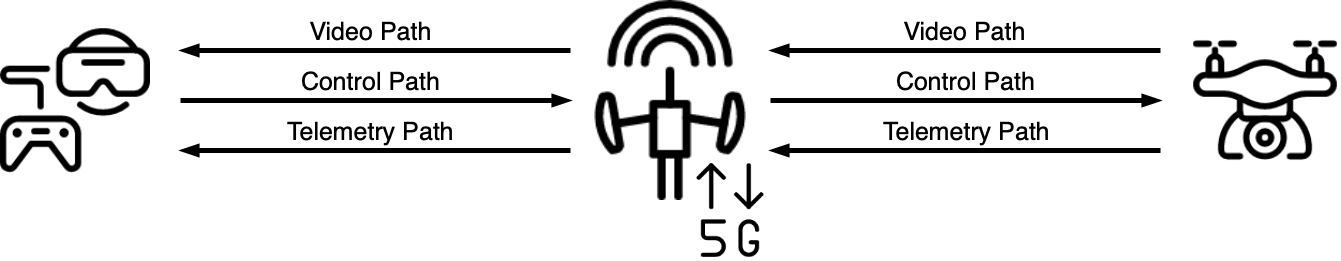
\includegraphics[width=1\textwidth]{templates/images/chapter04/use-case-scenario.png}
        \caption{Use Case Scenario}
        \label{fig:uc-scenario}
    \end{figure} 

In our use case we need to satisfy eMBB (to allow seamless video streaming) and uRLLC to enable an acceptable remote control of the vehicle.

\subsubsection {Video Path} 
The deployed 5G network must be able to successfully handle various video streams from the devices, satisfying bandwidth requirements. The user must be able to download (Rx) while the vehicle side must be able to upload (Tx) at similar rates to carry out the use case demo successfully. It goes without saying that the xNodeB should support at minimum these values in both directions. The values in Table \ref{tab:video-bw} are calculated by using 24 FPS which is considered acceptable for video streaming. Consequently, should the use case require true FPV or VR/AR, more FPS and/or higher quality, more bandwidth would be required.

\begin{table}[!ht]
   \begin{threeparttable}
\caption{Bandwidth in Relation to Video Quality}
\label{tab:video-bw}
\setlength\tabcolsep{0pt} % make LaTeX figure out intercolumn spacing

\begin{tabular*}{\columnwidth}{@{\extracolsep{\fill}} cl}
\toprule
     Bandwidth (Mbps)\tnote{1} & Usage scenario \\
\midrule
      0.5 &Minimum bandwidth required for live streaming \\
\addlinespace
     1.5 &Minimum bandwidth required for a broadband connection \\
\addlinespace
      3.0 &Standard Definition (SD) bandwidth \\
\addlinespace
      5.0 &High Definition (HD) bandwidth \\
\addlinespace
      25 &Ultra HD (4K UHD) bandwidth \\
\bottomrule
\end{tabular*}

\smallskip
\scriptsize

\begin{tablenotes}
\RaggedRight
\item[1] Due to uRLLC and eMBB characteristics, the UC1 should be executed in a customised network slice. Until this service offering becomes available in the Greece portfolio, UC1 will be executed (with some limited performance and/or functionality) in eMBB and uRLLC network slices offered as a service to the CSC.
\end{tablenotes}
   \end{threeparttable}
\end{table}
    
\newpage    
    
\subsubsection {Telecommand Path}
Depending on the type of vehicle used, the 5G solution should exhibit the same or less latency of transmission and reception of commands than traditional radio control solutions. This would allow for a paradigm shift in either reduced latency, theoretically unlimited range or both, over legacy systems.

\subsubsection {Telemetry Path}
The telemetry path aims to showcase an optional implementation of a mIoT slice for a less-demanding path in terms of network resources. Telemetry data such as drone location, altitude and orientation would prove extremely vital for flight path logging, as well as any potential use case specific sensors that could be mounted to the drone platform at each time.

%\newpage

\section {System Architecture Overview}
A more thorough description of the use case is provided on the next sections. Please note that final implementation concepts or hardware can vary, but the overall system architecture will remain the same.
\newpage
\subsection {User Side}
For the User Side, a configuration as shown in Figure \ref{fig:detailed-approach-user} is proposed:

    \begin{figure}[!ht]
        \centering
        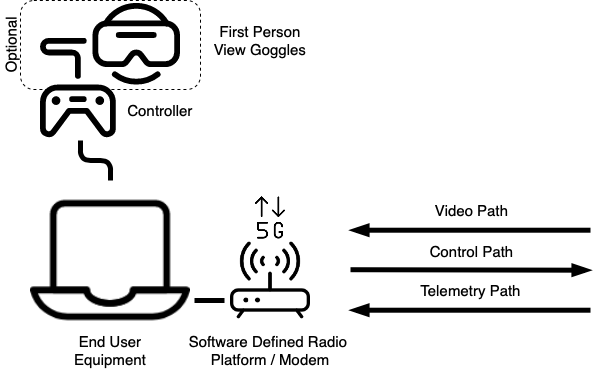
\includegraphics[width=0.9\textwidth]{templates/images/chapter04/detailed-approach-user.png}
        \caption{Detailed Approach for User Side of Use Case}
        \label{fig:detailed-approach-user}
    \end{figure} 

In our use case scenario, the goggles are replaced with a laptop for the sake of simplicity. This is in part for removing an extra layer of complexity from the development cycle and mainly for the reason that no 5G-compatible standalone headsets exist commercially. Most of the currently available products either use radio frequencies on the 2.4 or 5.8 GHz bands, suffering of course greatly from reduced range and reception quality. In future iterations, the First Person View goggles could be connected to a video out port on the end user equipment (in this case a laptop) to alleviate this problem. 
Due to the nature of analog control of vehicles, the laptop keyboard should be avoided as a means of steering at all costs, as it would prove too "rough" of an input device (either full throttle or none). For this reason, a wireless adapter will be used to relay a traditional two-stick radio controller's commands to the ground station software running on the laptop. Commercial joysticks aimed for video game use have demonstrated allot of jitter on their input so they are also disqualified for the sake of safety of both the drone and the pilot.
%In terms of processing power, the laptop could possibly be replaced with a thin client, for the sole reason that only decoding of the incoming video stream and transmission of low-bandwidth control commands would be required. %Greater attention should be put onto its networking capabilities and quality of screen for outdoor scenarios, but this is outside of the scope of this work.

\subsection {Vehicle Side}
Regarding the vehicle side, the following setup is proposed:

    \begin{figure}[!ht]
        \centering
        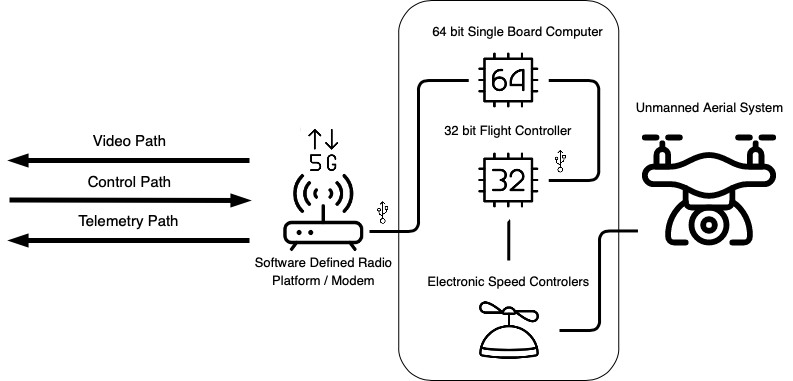
\includegraphics[width=1\textwidth]{templates/images/chapter04/detailed-approach-vehicle.png}
        \caption{Detailed Approach for Vehicle Side of Use Case}
        \label{fig:detailed-approach-vehicle}
    \end{figure} 

One of the most important parts of the use case is the vehicle side implementation. This is because all workload-intensive tasks such as video encoding and streaming while maintaining timely reaction to received commands are vital to its operation. For this reason, commercial off-the-shelf solutions that are geared towards recreational usage prove to be severely incapable of conforming to our platform needs. After extensive market research, only two solutions satisfied all the demands that our use case would require, those being either a custom-made solution from readily available parts or a drone research kit offered by Intel. Both of those proved to have their own distinct advantages, but the Ready to Fly (RtF) solution was preferred over the tedious task of tinkering with PID controllers and troubleshooting hardware bugs.
In short, the Intel Aero platform provides a powerful, yet light enough Single Board Computer (SBC) for video encoding and streaming, as well as a combined takeoff weight of 1.9kgs. This would allow for more than enough headroom for future expansions, as additional cameras or sensors and easily be mounted and still maintain nominal 20 minutes flight time. Finally, the kit comes bundled with Intel's own flight controller, that connects over a serial port to the companion computer.% and offers the ability to send and receive control commands over any network or interface, proving especially useful for our implementation.

\newpage

\section {Intermediate Implementation Steps}
\subsubsection {Step 1}
%The setup seen on Figure \ref{fig:impl-step1} could be used at the first phase of implementation
By only using laptops, the first step ensures the integrity of communication between the UE through the experimental cellular network.

    \begin{figure}[!ht]
        \centering
        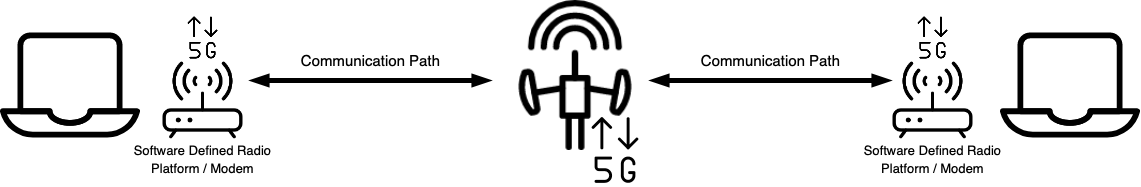
\includegraphics[width=0.9\textwidth]{templates/images/chapter04/impl-step-01.png}
        \caption{Implementation Step 1 - Verify Communication}
        \label{fig:impl-step1}
    \end{figure} 

\subsubsection {Step 2}
Using the same setup as before, replacing data with a complete video streaming pipeline between the UE and ground station in order to verify its quality.

    \begin{figure}[!ht]
        \centering
        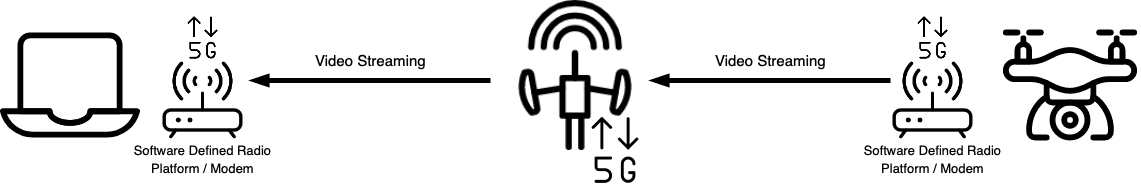
\includegraphics[width=0.9\textwidth]{templates/images/chapter04/impl-step-02.png}
        \caption{Implementation Step 2 - Verify Streaming}
        \label{fig:impl-step2}
    \end{figure}
    
\subsubsection {Step 3}
Finally, replacing the laptop with a \acrfull{sbc}, will allow to verification of the minimum system requirements. Simultaneously, the flight controller module can be also tested to verify cohesion of the control path.

    \begin{figure}[!ht]
        \centering
        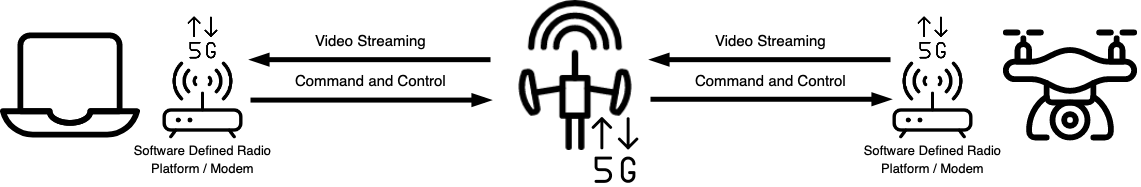
\includegraphics[width=0.9\textwidth]{templates/images/chapter04/impl-step-03.png}
        \caption{Implementation Step 3 - \acrshort{sbc} Requirements and Remote Control}
        \label{fig:imple-step3}
    \end{figure} 
\newpage

\section {Suggested Hardware}
The combination of digital processing and analog RF has always made up communication systems. In today's modern systems signal processing has progressed to such an extent that a majority of baseband functionality is being implemented in software. The flexibility of the RF hardware to be re purposed and reconfigured has led to one radio font-end handling most RF systems. Normally the RF front-end is software controlled rather than software defined. This modern combination of flexible RF front-ends and signal processing in software has lead to the birth of software-defined radio. In general, a digital communications system consists of an interdependent sequence of operation responsible for taking some type of information and transmits it over-the-air to a receiver for processing and decoding into a reconstructed version of the original information signal.

There has been a growing amount of interest with respect to combining SDR technology with software-defined networks (SDNs), where the latter focuses on adapting the higher communication layers to the prevailing operational environment. This enables things like modification of the routing to be tied to heuristiccs provided by the physical layers. 

Next-generation communications systems introduce new challenges that require solutions beyond what can be achieved through individual device optimization. Integrating more software control and cognitive abilities to the radio demands a more frequency- and bandwidth-flexible RF design. To achieve this goal static filters need to be removed and replaced with tunable filters. Similarly, the concept of a common platform would allow for shorter development times, reduced manufacturing costs, and provide greater interoperability between systems. The common platform demands that the RF system be capable of providing full performance for applications that traditionally had very different architectures. Finally, future platforms are pushing size and power demands to a new extreme.

\subsection {Suggested Hardware for xNodeB}
For this reason design considerations to take into account when devising digital communication systems based on an SDR platform include the integration of the physical and network layers via a real-time protocol implementation of an embedded processor. Most communication systems are divided into logically separated layers in order to more readily facilitate the design of the communication system. However, it is imperative that each layer is properly designed due to the strong interdependence between all the layers. Ensuring that a sufficiently wide bandwidth radio front-end exists with agility over multiple subchannels and a scalable number of antennas for spatial processing. Many networks employing digital communication systems possess a centralized architecture for controlling the operations of the overall network. Knowing the radio network architecture is important since it will dictate what sort of operations are essential for one digital transceiver to communicate with another. The ability to perform controlled experiments in different environments is important for the sake of demonstrating the reliability of a particular SDR implementation, providing a sanity check capability. Reconfigurability and fast prototyping through a software design flow for algorithm and protocol description. 

From the perspective of a radio system and its implementation, much of the system design will focus on the physical layer, but it can't be forgotten how the link layer may affect the physical. Nevertheless, given that the baseband processing is all conducted in software, it is possible for the communications system to implement the higher layers of the stack in software as well. Many communication standards have adopted this scheme, where the entire communication system across all the layers are implemented in software, although depending on data rate requirements, this can require significant computational capabilities on the part of the system to achieve real-time operation. All software implementation enable functional updates without hardware replacements.The trade-offs of which function or layer is done in fixed hardware versus flexible software is an engineering decision based on volume, cost , power, complexity and many other factors. 
%software defined radio for engineers, p.8

\begin{sidewaystable*}
    \begin{threeparttable}
    \scriptsize
        \caption{Software Defined Radio Platforms for xNodeB}
        \label{tab:sdr-xnodeb}
    \begin{tabularx}{\textwidth}{@{}l*{10}{C}c@{}}
    \addlinespace
    \toprule
     & Range (MHz) & Bandwidth (MHz) & Rx/Tx & Duplex & Tx Power (dBm) & Sampling (MSps) & Interface & Chipset (FPGA) &  Gates (K) & Size (mm)  & Price (USD)\\ 
     \addlinespace
        \midrule
        \addlinespace 
        USRP N210 & - & - & - & - & 15 & 100 & 1x 1Gb & DSP3400 & 6 & Half RU & 2,048\\  
        USRP N300 & 10 - 4400 & 100 & 2/2 & Full & 18 & 153.6 & 2x SFP+ & Zynq7035 & 275 & Half RU & 6,850\\ 
        USRP N310 & 10 - 6000 & 100 & 4/4 & Full & 18 & 153.6 & 2x SFP+ & Zynq7100 & 444 & Half RU & 10,537\\ 
        USRP N320 & 3 - 6000 & 200 & 2/2 & Half & 18 & 153.6 & 1xQSFP+ & Zynq7100 & 444 & Half RU & 12,000\\
        USRP N321 & 3 - 6000 & 200 & 2/2 & Half & 18 & 153.6 & 1xQSFP+ & Zynq7100 & 444 & Half RU & 13,500\\
        \addlinespace
        USRP X300 & - & - & - & - & 10 & 200 & 2x10Gb & XC7K325T & 326 & 277x218x39 & 4,640\\
        USRP X310 & - & - & - & - & 10 & 200 & 2x10Gb & XC7K410T & 407 & 277x218x39 & 5,714\\  
        \addlinespace
        USRP E310 & 70 - 6000 & 56 & 2/2 & Full & 10 & 61.44 & 1x1Gb & Zynq7020 & 85 & 133x68.2x26 & 3,221\\
        USRP E313 & 70 - 6000 & 56 & 2/2 & Full & 10 & 61.44 & 1x1Gb & Zynq7020 & 85 & 186x280x106 & 4,334\\
        \addlinespace
        LimeSDR & 0.1 - 3800 & 61.44 & 2/2 & Full & 10 & 61.44 & USB 3.0 & Cyclone 4 & 40 & 100x60 & 315\\
        LimeSDR QPCIe & 0.1 - 3800 & 61.44 & 4/4 & Full & 10 & 61.44 & PCIe x4 & Cyclone 4 & 80 & 136,85x68,9 & 799\\
        LimeNET Micro & 0.1 - 3800 & 61.44 & 2/2 & Full & 10 & 61.44 & USB 2.0 & Cyclone 4 & 40 & 125x65 & 345\\
        LimeNET Mini & 0.1 - 3800 & 61.44 & 2/2 & Full & 10 & 61.44 & 1x 1Gb & Cyclone 4 & 40 & 110x105 & 2,799\\
        LimeNET Base Station & 0.1 - 3800 & 61.44 & 4/4 & Full & 10 & 61.44 & 2x 1Gb & Cyclone 4 & 40 & 265x270x260 & 21,250\\
        LimeNET CrowdCell & 0.1 - 3800 & 61.44 & 2/2 & Full & 10 & 61.44 & 1x 1Gb & Cyclone 4 & 40 & N/A & N/A\\
        \addlinespace
        \midrule
        \addlinespace
        SBX 782761 & 400 - 4400 & 40 & 1/1 & Full & - & - & - & - & - & - & 573\\  
        SBX 783351 & 400 - 4400 & 120 & 1/1 & Full & - & - & - & - & - & - & 688\\  
        \addlinespace 
        CBX 782760 & 1200-6000 & 40 & 1/1 & Full & - & - & - & - & - & - & 573\\ 
        CBX 783353 & 1200-6000 & 120 & 1/1 & Full & - & - & - & - & - & - & 688\\
        \addlinespace 
        UBX 783774-01 & 10 - 6000 & 40 & 1/1 & Full & - & - & - & - & - & - & 1,056\\  
        UBX 783775-01 & 10 - 6000 & 160 & 1/1 & Full & - & - & - & - & - & - & 1,291\\
        \addlinespace 
        TwinRX & 10 - 6000 & 80 & 2/0 & Half & - & - & - & - & - & - & 2,890\\
        \addlinespace
        \midrule
    \end{tabularx}
    \begin{tablenotes}
        \RaggedRight
        \item[1] https://www.intel.com/content/dam/www/programmable/us/en/pdfs/literature/pt/cyclone-iv-product-table.pdf.
        \item[2] Amplification.
        \item[3] Max stated, may vary in MIMO configuration .
        \item[4] additional daughterboards required.
        \item[5] small cell form-factor.
    \end{tablenotes}

    \end{threeparttable}
\end{sidewaystable*}

The USRP N310 is a networked software defined radio (SDR) that provides reliability and fault-tolerance for deployment in large-scale and distributed wireless systems. It simplifies control and management of a network of radios by introducing the unique capability to remotely perform tasks such as updating software, rebooting, factory resetting, self-testing, host PC/ARM debugging and monitoring system health. The USRP N310 is one of the highest channel density devices in the SDR market, offering four RX and four TX channels in a half-wide RU form factor. The RF front end uses two AD9371 transceivers, the latest RFIC technology from Analog Devices. Each channel provides up to 100 MHz of instantaneous bandwidth and covers an extended frequency range from 10 MHz to 6 GHz. The open-source USRP Hardware Driver (UHD) API and RF Network-on-Chip (RFNoC) FPGA development framework reduces software development effort and integrates with a variety of industry-standard tools. The baseband processor uses the Xilinx Zynq-7100 SoC to deliver a large user-programmable FPGA for real-time and low-latency processing and a dual-core ARM CPU for stand-alone operation. Users can deploy applications directly on to the preinstalled embedded Linux operating system or stream samples to a host computer using high-speed interfaces such as 10 Gigabit Ethernet over the two SFP+ ports.

Additionally, the USRP N310 has a flexible synchronization architecture with support for traditional SDR synchronization methods such as clock reference, PPS time reference, and GPSDO, which enable implementation of high channel count MIMO systems. In addition, the USRP N310 uniquely features Ethernet-based synchronization using the open-source White Rabbit timing protocol which enables precise baseband synchronization over large distances in GPS-denied environments. All Ettus Research USRP SDRs and NI USRP SDRs are supported by the USRP Hardware Driver, which is published by NI under open-source licenses. This driver facilitates application development on USRP hardware and offers cross-platform support for multiple industry-standard development environments and frameworks. As dual-licensed software, the USRP Hardware Driver is available under the open-source GNU General Public License version 3 (GPLv3).%ni.com/sdr blabla & N310 product page

\begin{figure}
    \centering
    \subfloat[Isometric view of the N310]{
      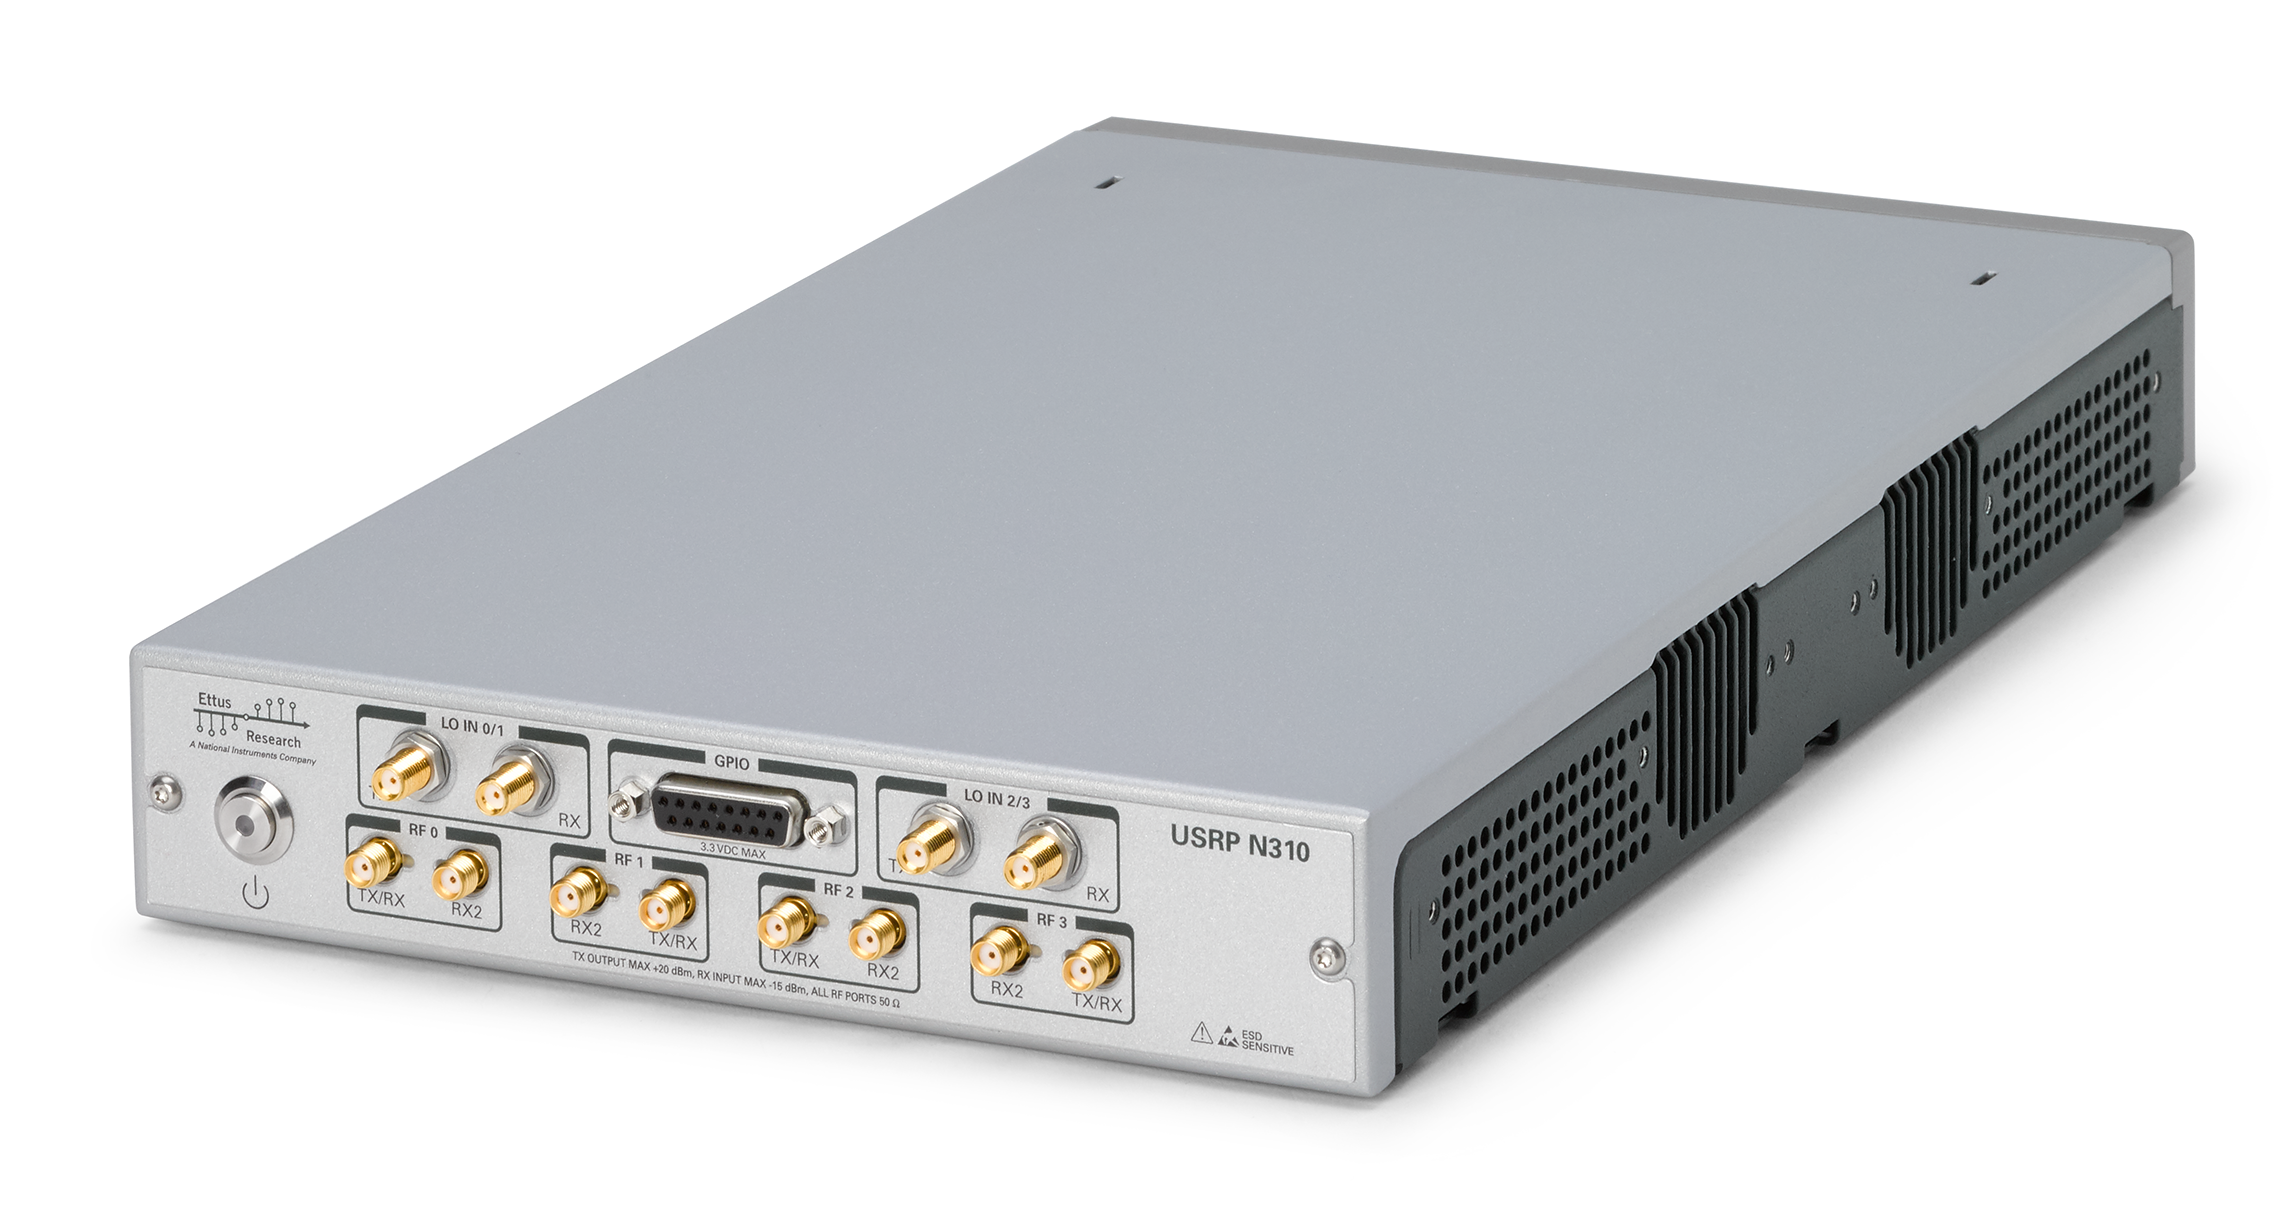
\includegraphics[width=0.9\textwidth]{templates/images/chapter05/N310_Iso-e1550871338956.png}%
      }\par
    \subfloat[Front side connectors]{%
      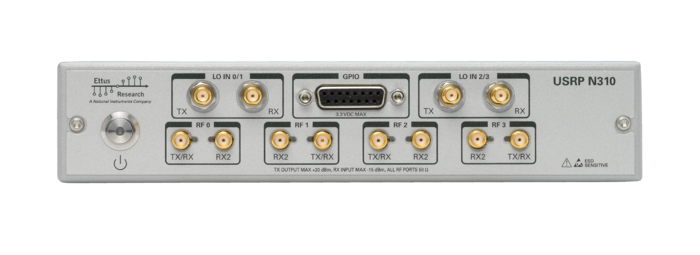
\includegraphics[width=0.9\textwidth]{templates/images/chapter05/700px-n310_front.png}%
      }\par        
    \subfloat[Back side connectors]{%
      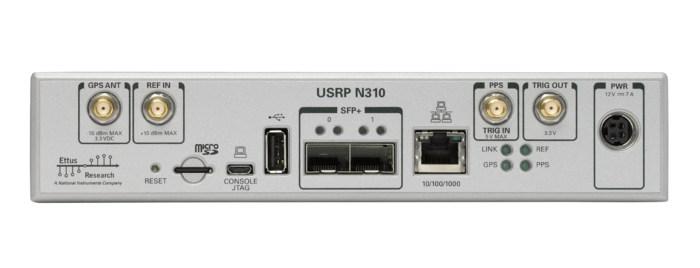
\includegraphics[width=0.9\textwidth]{templates/images/chapter05/700px-n310_back.png}%
      }
    \caption{View of the N310 SDR platform. Source: \cite{ettus-n310}}
    \label{TS}
\end{figure}
    
\newpage
%\subsection {Suggested Hardware for User Side}
%Handheld radios are becoming more capable and complex, but simultaneously requiring improved battery efficiency. Small UAVs lack the power generation of large aircraft and every milliwatt that the RF system consumes directly translates to payload battery weight, and thus, reduced flight time. To overcome these challenges and create the next generation of aerospace and defense solutions, a new radio architectures are being developed.
%Since its inception, the superheterodyne architecture has been the backbone of radio design. Whether it is a handheld radio, unmanned aerial vehicle (UAV) data link, or a signal intelligence receiver, the single or dual mixing stage superheterodyne architecture is the common choice with significant gains in performance across the entire signal chain. Microwave and RF devices have improved their performance while decreasing power consumption. ADCs and DACs have increased the sample rate, linearity, and effective number of bits (ENOB). Processing capability in FPGAs and DSPs have abide by Moore’s law, allowing for more efficient algorithms, digital correction, and further integration. Package technology has shrunk device pin density while simultaneously improving thermal handling.
%However, these device-specific improvements are beginning to reach the point of diminishing returns. While the RF components have followed a reduced size, weight, and power (SWaP) trend, high-performance filters remain physically large and are often custom designs, adding to overall system cost. Additionally, the IF filters set the analog channel bandwidth of the platform, making it difficult to create a common platform design that can be reused across a wide range of systems. For package technology, most manufacturing lines will not go below a sub-mm ball pitch, placing a limit on how physically small a complex device with many I/O requirements can become.
%software defined radio for engineers, p.10

%\begin{sidewaystable*}
%    \begin{threeparttable}
%    \scriptsize
%        \caption{Software Defined Radio Platforms for }
%        \label{tab:sdr-ue}
%    \begin{tabularx}{\textwidth}{@{}l*{10}{C}c@{}}
%    \addlinespace
%    \toprule
%     & Frequency Range(MHz) & Channel BW(MHz) & Rx/Tx & Duplex (Full/Half) & N. Figure  (dB) & Sample  (MSps) & Interface & Chipset (FPGA) &  Gates (k) & Size (mm)  & Price  \\ 
%     \addlinespace
%        \midrule
%        \addlinespace 
%        USRP B200 & 70-6000 & 56 & 1/1 & Full & 8 & 61,44 & USB 3.0 & XC6SLX75 & 75 & 97x155x15 & 785\\
%        USRP B210 & 70-6000 & 56 & 2/2 & Full & 8 & 61,44 & USB 3.0 & XC6SLX150 & 147 & 97x155x15 & 1,282\\
%        \addlinespace 
%        USRP B200mini & 70-6000 & 56 & 1/1 & Full & 8 & 61,44 & USB 3.0 & XC6SLX75 & 75 & 83.3x50.8x8.4 & 807\\
%        USRP B200mini-i & 70-6000 & 56 & 1/1 & Full & 8 & 61,44 & USB 3.0 & XC6SLX75 & 75 & 83.3x50.8x8.4 & 932\\
%        USRP B205mini-i & 70-6000 & 56 & 1/1 & Full & 8 & 61,44 & USB 3.0 & XC6SLX150 & 147 & 83.3x50.8x8.4 & 959\\
%        \addlinespace 
%        LimeSDR & 10 - 3800 & 61.44 & 2/2 & Full & 3.5 & 61.44 & USB 3.0 & Cyclone 4 & 40 & Vendor & 315\\
%        LimeSDR Mini & 10 - 3500 & 30.72 & 1/1 & Full & 3.5 & 30.72 & USB 3.0 & MAX 10 & 16 & 69x31.4 & 175\\
%        \addlinespace 
%        XTRX CS & 30 - 3700 & 120 & 2/2 & Full & 3.5 & 3.5 & PCIe x2 &  XC7A35T & 33 & Mini PCIe & 260\\
%        XTRX Pro & 30 - 3700 & 120 & 2/2 & Full & 3.5 & 3.5 & PCIe x2 &  XC7A50T & 52 & Mini PCIe & 599\\
%        \addlinespace
%        \midrule
%    \end{tabularx}
%    \begin{tablenotes}
%        \RaggedRight
%        \item[1] For users in vehicles, the UE can be connected to the network directly, or via an on-board moving base station.
%        \item[2] A certain traffic mix is assumed; only some users use services that require the highest data rates [2].
%        \item[3] For interactive audio and video services, for example, virtual meetings, the required two-way end-to-end latency (UL and DL) is 24 ms while the corresponding experienced data rate needs to be up to 8K 3D video [300 Mbps] in uplink and downlink.
%        \item[4] These values are derived based on overall user density. Detailed information can be found in [10].
%    \end{tablenotes}

%    \end{threeparttable}
%    \end{sidewaystable*}
\newpage
%\subsection {Suggested Hardware for Vehicle Side}
%<*Intel Aero>

%MAVLink or Micro Air Vehicle Link is a protocol for communicating with small unmanned vehicle. It is designed as a header-only message marshaling library. MAVLink was first released early 2009 by Lorenz Meier under LGPL license. It is used mostly for communication between a Ground Control Station (GCS) and Unmanned vehicles, and in the inter-communication of the subsystem of the vehi- cle. It can be used to transmit the orientation of the vehicle, its GPS location and speed.
%This will be the primary means of communication between the onboard computer and the dedicated autopilot module. [https://www.intel.com/content/dam/support/us/en/documents/boardsandkits/aero/ apu-161110-pixhawk-flight-guide.pdf] This way, the user will be able to control the vehicle remotely with a simple TCP or UDP connection, as-well as get instant telemetry feedback, by configuring ap- propriately the autopilot’s ports. [http://ardupilot.org/copter/docs/common-telemetry-port-setup-for- apm-px4-and-pixhawk.html]

\newpage

\section {Bill of Materials (BOM)}

\begin{table}[H]
   \begin{threeparttable}
\caption[Suggested Bill of Materials] {(BOM)}
\label{tab:equipment-list}
\setlength\tabcolsep{0pt} % make LaTeX figure out intercolumn spacing

\begin{tabular*}{\columnwidth}{@{\extracolsep{\fill}} lcS[table-format=-3.2]}
    \toprule
         Parts list\tnote{a} & Quantity\tnote{\emph{b}} & Cost\\
\addlinespace
\addlinespace
    Autopilot + Processing&&\\
\cmidrule{1-1}
    Pixhawk 4 + PM07&1&215.00\\
    Intel Aero board &1 &399.00\\
    Intel Aero enclosure &1 &69.00\\
    Inter Aero vision kit &1 &149.00\\
    USB OTG adapter &1 &16.00\\
\addlinespace
\midrule
    TOTAL & & \\
\midrule    
    
\addlinespace
\addlinespace
    Wireless Communications&&\\
\cmidrule{1-1}
    Wireless Communications &&\\
    LimeSDR Mini&2&318.00\\
    High Gain Omni Antenna&2&50.00\\
    LimeNET Base Station&1&21250.00\\
\midrule
    TOTAL&&\\
\midrule
    
\addlinespace
\addlinespace
    Hardware Total &&\\
\addlinespace
    GRAND TOTAL&&\\
\bottomrule
\end{tabular*}

\smallskip
\scriptsize

\begin{tablenotes}
\RaggedRight
\item[1] Due to uRLLC and eMBB characteristics, the UC1 should be executed in a customised network slice. Until this service offering becomes available in the Greece portfolio, UC1 will be executed (with some limited performance and/or functionality) in eMBB and uRLLC network slices offered as a service to the CSC.
\end{tablenotes}
   \end{threeparttable}
\end{table}

%3GPP_Rel_13_15_Final_to_Upload_2.28.17_AB